% BEGIN_FOLD preamble

\documentclass{article}
\usepackage[activeacute,spanish]{babel}
\usepackage{lmodern}
\usepackage[T1]{fontenc}
\usepackage{url,multirow}
\usepackage[centertableaux,smalltableaux]{ytableau}
\usepackage[utf8]{inputenc}
\usepackage{cancel, comment}
\usepackage[left=2cm,top=1.5cm,right=2cm, bottom=1.5cm,letterpaper, includeheadfoot]{geometry}
\usepackage{amssymb, amsmath, amsthm, mathtools}
\usepackage{graphicx}
\usepackage{hyperref}
\hypersetup{
	colorlinks,
	linkcolor={red!50!black},
	citecolor={blue!50!black},
	urlcolor={blue!80!black}
}

\usepackage[prependcaption,textsize=tiny,,textwidth=5cm]{todonotes}
\newcommand{\js}[1]{\todo[inline,linecolor=red,backgroundcolor=red!25,bordercolor=red]{jsoto. #1}}

\usepackage{paralist}
\usepackage{contour}
\usepackage{algorithm, algorithmic}

%%%Definiciones
\newcommand{\dis}{\displaystyle}
\newcommand{\IV}[1]{[\![#1]\!]} %Iverson

\newcommand{\E}{\mathcal{E}}
\newcommand{\V}{\mathcal{V}}

\def\multiset#1#2{\ensuremath{
		\mathchoice{\left(\kern-.3em\left(\genfrac{}{}{0pt}{}{#1}{#2}\right)\kern-.3em\right)}}
	{\big(\!\binom{#1}{#2}\!\big)}{\big(\!\binom{#1}{#2}\!\big)}{\big(\!\binom{#1}{#2}\!\big)}}
\DeclareRobustCommand{\sbinom}{\genfrac{[}{]}{0pt}{}}
\DeclareRobustCommand{\lbinom}{\genfrac{\{}{\}}{0pt}{}}
\newcommand{\fallfac}[2]{{#1}^{\underline{#2}}}
\newcommand{\risefac}[2]{{#1}^{\overline{#2}}}

\newcommand{\defn}[1]{\textit{\textsc{[Def]\,}}\textbf{#1}\\[5pt]\indent}
\newcommand{\nin}{\noindent}
% macros
\newcommand{\QQ}{\mathbb Q}
\newcommand{\RR}{\mathbb R}
\newcommand{\NN}{\mathbb N}
\newcommand{\ZZ}{\mathbb Z}
\newcommand{\FF}{\mathbb F}
\newcommand{\CC}{\mathbb C}
\newcommand{\EE}{\mathbb E}
\DeclareMathOperator{\COM}{COM}
\DeclareMathOperator{\com}{com}
\DeclareMathOperator{\ord}{ord}
\DeclareMathOperator{\DFJ}{DFJ}
\DeclareMathOperator{\EUL}{EUL}
\DeclareMathOperator{\WCOM}{WCOM}
\DeclareMathOperator{\wcom}{wcom}
\newcommand{\sop}{\operatorname{sop}}

%Teoremas, Lemas, etc.

\theoremstyle{plain}
\newtheorem{teo}{Teorema}
\newtheorem{lem}[teo]{Lema}
\newtheorem{prop}{Proposici\'on}
\newtheorem{cor}[teo]{Corolario}
\newtheorem{cor*}{Corolario}
\theoremstyle{definition}
\newtheorem{defi}[teo]{Definici\'on}
\newtheorem{eje}[teo]{Ejemplo}
\newtheorem{ejeres}[teo]{Ejercicios resueltos}
\newtheorem{ejere}[teo]{Ejercicio resuelto}
\newtheorem{ejes}[teo]{Ejemplos}
\newtheorem{ejer}[teo]{Ejercicio}
\newtheorem{prob}[teo]{Problema}
\newtheorem{obs}[teo]{Observaci\'on}
\newtheoremstyle{Azul}
{\topsep}   % ABOVESPACE
{\topsep}   % BELOWSPACE
{\color{blue}}  % BODYFONT
{0pt}       % INDENT (empty value is the same as 0pt)
{\color{blue}\bfseries} % HEADFONT
{.}         % HEADPUNCT
{5pt plus 1pt minus 1pt}  % HEADSPACE. `plain` default: {5pt plus 1pt minus 1pt}
{}          % CUSTOM-HEAD-SPEC
\theoremstyle{Azul}
\newtheorem*{comm}{Comentario}
\newcommand{\commento}[1]{\noindent{\color{blue}#1}\vspace*{-3pt}}

% fin macros

\usepackage{fancyhdr}
\pagestyle{fancy}
\fancypagestyle{plain}{%
\fancyhf{}
\lhead{\footnotesize\itshape\bfseries\rightmark}
\rhead{\footnotesize\itshape\bfseries\leftmark}
}

% END_FOLD
\begin{document}
% BEGIN_FOLD encabezado
\setlength{\headheight}{14pt}
\fancyhead[L]{Facultad de Ciencias F\'isicas y Matem\'aticas}
\fancyhead[R]{Universidad de Chile}
\vspace*{-1.2 cm}
\begin{minipage}{0.6\textwidth}
	\begin{flushleft}
		\hspace*{-0.5cm}\textbf{MA4702. Programación Lineal Mixta 2020.}\\
		\hspace*{-0.5cm}\textbf{Profesor: José Soto.}\\
	\end{flushleft}
\end{minipage}
\begin{minipage}{0.36\textwidth}
	\begin{flushright}
		
\includegraphics[scale=0.15]{fcfm.pdf}
	\end{flushright}
\end{minipage}
\bigskip
%Fin encabezado

% END_FOLD
\newif\ifsol
\soltrue
\solfalse

\begin{center}
  \LARGE \textbf{Tarea 4}.\\
\end{center}
\bigskip

\noindent\textbf{Fecha entrega}: Lunes 13 de Julio, 23:59. Por u-cursos.
\subsection*{Instrucciones:} 
\begin{enumerate}
\item \textbf{Extensión máxima}: Entregue su tarea en a lo más \textbf{6 planas}.
    \item \textbf{Formato:} La tarea debe entregarse en formato pdf, con fondo de un solo color (blanco de preferencia), letra legible en manuscrito y clara. (No se aceptarán documentos tipeados o generados por computador, pero si tiene alguna manera de escribir en manuscrito directamente de manera digital lo puede hacer).
    Si desarrolla su tarea en papel, entréguelo escaneados o en fotos de alta calidad, via ucursos.    \item \textbf{Tiempo de dedicación:} El tiempo estimado de \emph{desarrollo} de la tarea es de 3 horas de dedicación. Esto no considera el tiempo de estudio previo, el tiempo dedicado en asistir a cátedras y auxiliares, ni el tiempo para \emph{ponerse al día}. \textbf{En particular, para la última parte se recomienda repasar la clase 19 del curso}.
     Tendrá un plazo de 7 días para entregarlo. No espere hasta el último momento para escanear o fotografiar adecuadamente su tarea y cambiarla al formato solicitado (pdf). Entregue con suficiente anticipación a la hora límite.
    \item \textbf{Revisión:} Se podrá descontar hasta 1 punto en la nota final por falta de formato o extensión.
\item Esta tarea está pensada para ser hecha en forma individual.
    \end{enumerate}
    
  \subsection*{Definiciones para esta tarea}
Sea $N$ un conjunto finito. Decimos que dos conjuntos $A, B \in 2^N$ son \emph{intersectantes} si los conjuntos $A\setminus B$, $B\setminus A$ y $A\cap B$ son todos no vacíos. Notamos que cuando dos conjuntos no son intersectantes entonces debemos tener que $A$ y $B$ son disjuntos, o bien uno contiene al otro.

Una familia $\mathcal{L}\subseteq 2^N$ de subconjuntos de $N$ se dice \textbf{familia laminar sobre $N$} si no posee pares de conjuntos intersectantes, es decir, si para todo $A, B\in \mathcal{L}$.
\begin{align*}
(A\subseteq B) \text{ o } (B\subseteq A) \text{ ó } 
(A\cap B = \emptyset)
\end{align*}


\subsection*{Ejercicios:}
\noindent \textbf{Parte I (30 puntos).} \textbf{Elija, resuelva y entregue 3 ejercicios de esta parte $I$.} Si entrega más que 3 se calificarán los 3 peores ejercicios entregados.
\begin{enumerate}[(a)]
\item Demuestre la siguiente dirección del Teorema de Ghoulia-Houri: 
Si $A\in \{-1,0,1\}^{m\times n}$ es una matriz totalmente unimodular, entonces para todo $J\subseteq [n]$ existe una partición $J_1, J_2$ de $J$ tal que
$$\sum_{j\in J_1}a_{ij}-\sum_{j\in J_2}a_{ij} \in \{0,1,-1\}, \text{ para todo } i \in [m].$$
\textbf{Indicación:} Sea $B=A^J$. Demuestre que el poliedro $P=\{x\in \RR^J\colon \lfloor \frac12 B 1 \rfloor \leq Bx\leq \lceil \frac12 B 1\rceil, 0\leq x \leq 1\}$ es no vacío, y concluya que tiene un punto  $y\in \{0,1\}^J$ integral. Use ese punto $y$ para determinar la partición pedida (el vector $y$ tiene solo 2 tipos de valores).

\textbf{Solución}\\

$P$ es un polítopo no vacío, en efecto, si tomamos $x=\frac{1}{2}$ tenemos que $\lfloor \frac12 B 1 \rfloor \leq \frac{1}{2}B 1\leq \lceil \frac12 B 1\rceil$, luego el poliedro anterior se puede escribir como $Cx\leq b$, con $C =  [B\;|-B\;|\;I\;|\;-I]$ y $b=[\lfloor \frac12 B 1 \rfloor\;|-\!\lceil \frac12 B 1\rceil\;|\;1\;|\;0]^T$. Como $B$ es TU, $C$ también lo es. Además, como $b\in \mathbb{Z}^{2m+2|J|}$ es entero, se tiene que $P$ es entero y luego sus vértices son enteros. Además, usando que $B1 = \lfloor \frac 12 B1\rfloor + \lceil\frac 12 B1\rceil$, se tiene que para todo $x\in P$, $\lfloor \frac 12 B1\rfloor \leq B1 - Bx \leq \lceil \frac12 B1\rceil$, es decir $1-x\in P$. 
Sea entonces $y^1\in\{0,1\}^{J}$ un vértice de $P$, $J_{1}=\{j \in J| y^1_{j}=1\}$ y $J_{2}=\{j \in J| y^1_{j}=0\}$. Por lo anterior $y^2:=1-y^1$ también es punto integral de $P$ y luego para $k\in \{1,2\}$, e $i\in [m]$ se tiene 
$\sum_{j\in J_k}a_{ij}=(By^k)_i\in \{\lfloor\frac{1}{2}B1\rfloor_i, \lfloor\frac{1}{2}B1\rfloor_i\}$. Se concluye entonces que $$\sum_{j\in J_1}a_{ij}-\sum_{j\in J_2}a_{ij} \in \{0,1,-1\}, \text{ para todo } i \in [m].$$


\item Sea $\mathcal{I}$ una familia de intervalos cerrados, todos subconjuntos de $[0,n]$ y cada uno con sus extremos enteros. El \emph{minimum hitting set problem} consiste en encontrar el conjunto $H\subseteq [0,n]\cap \ZZ$ de menor cardinalidad tal que cada intervalo $J\in \mathcal{I}$ contiene al menos un punto de $H$. Encuentre un programa lineal puro que permita resolver este problema. \textbf{Indicación:} Demuestre primero que el programa lineal entero natural, tiene conjunto factible integral.

\textbf{Solución}

$H\subseteq \{0, 1, \ldots, n\} = [n]_0$, sea $x_{i}=1$ si $H$ contiene el elemento $i$, $0$ si no, luego el \textit{minimum hitting set problem} se puede escribir como un PLE como sigue:
\begin{align*}
    \min \sum_{i\in[n]_0}  x_{i}\\
    \sum_{i\in [n]_0|\;l\leq i\leq u}x_{i} & \geq 1\quad \forall [l,u] \in \mathcal{L}\\
    0\leq x_{i} &\leq 1 \quad \forall i\in [n]_0.\\
    x&\in \ZZ^{[n]_0}
\end{align*}
La primera restricción obliga a que $H$ contenga al menos un punto de cada intervalo cerrado $[l,u]$ de $\mathcal{L}$. El poliedro asociado a la relajación del PLE anterior se puede como escribir como $P = \{x\,|\, Mx\geq 1, 0\leq x\leq 1\}$, con $M\in \{0,1\}^{[n]_0\times\mathcal{L}}$, donde $M_{i,[l,u]}=1$ si $l\leq i\leq u$. Notar que de un intervalo $[l,u]\in \mathcal{L}$ solo nos interesa la parte entera, es decir, $\{l, l+1, \ldots, u-1, u\}$. Si enumeramos las filas desde el $0$ se tiene que $M_{l, [l,u]}=M_{l+1, [l,u]} = \ldots,M_{u-1, [l,u]}= M_{u, [l,u]}=1$ y $M_{i, [l,u]}=0 \; \forall i \notin \{l, l+1, \ldots, u-1, u\}$. Por ende, la matriz $M$ tiene la propiedad de los $1$'s consecutivos a nivel columna, por lo que $M$ es TU, además, como el lado derecho es entero se tiene que $P$ es integral. Por último, se tiene que $P$ es no vacío ($x=1\in P$), y es un polítopo ($0\leq x\leq 1$), por tanto, alcanza su óptimo en un vértice $x^{*}$ y como $P$ es integral el vértice es entero, por lo que $H=\{i\in[n]|x^{*}_{i}=1\}$ es el $\textit{minimum hitting set}$.

\item Sea $A\in \RR^{m\times n}$, con $m\leq n$. Demuestre que $A$ es totalmente unimodular si y solo si $[A | I]$ es unimodular.

\textbf{Solución}

\textbf{($\Longrightarrow$)} Si $A$ es TU se tiene que toda submatriz cuadrada de $A$ tiene determinante en $\{-1,0,1\}$. Sea $B$ una submatriz cuadrada maximal de $[A|I]$ con $J$ el subconjunto de columnas asociadas, con $|J|=m$, si todas las columnas pertenecen a $A$ o $I$ se tiene que $B$ es TU ya que ambas lo son, si tiene columnas de $A$ e $I$ podemos construir $B'$ a partir de $B$, donde $B'$ tiene todas las columnas de $A$ a la izquierda y todas las de $I$ a la derecha seguido de una permutación de filas tal que:

\[
B'=
\left[
\begin{array}{cc}
B_{2} & 0 \\
B_{1} & I_{B}
\end{array}
\right],
\]
donde $B_{1}$ y $B_{2}$ son submatrices de $A$ y $B_{2}$ es cuadrada, luego se tiene que $det(B')=\det(B_{2})\in \{-1, 0, 1\}$, se concluye que toda submatriz maximal de $[A|I]$ tiene determinante en $\{-1,0,1\}$ por lo que $[A|I]$ es UNI.

\textbf{($\Longleftarrow$)} Sea $B_{2}$ una submatriz cuadrada de $A$, supongamos que no es maximal, luego $B_{2}$ la podemos completar con una submatriz $B_{1}$ de $A$ y columnas de $I$ para formar la misma matriz maximal $B'$ de $[A|I]$ del punto anterior, por ende, se tiene que $\det(B') \in \{-1, 0, 1\}$ ya que $[A|I]$ es UNI, luego $\det(B') = \det(B_{2})\det(I) = \det(B_{2})$, se concluye que toda submatriz cuadrada de $A$ tiene determinante en $\{-1,0,1\}$, por tanto, $A$ es TU.


\item Sea $G=(V,E)$ un digrafo, y sean $s$, $t$ dos nodos distintos de $V$. Encuentre un programa lineal puro que permita resolver el problema del $s$-$t$ camino de largo (número de aristas) mínimo.\\ \textbf{Indicación:} Escriba primero este problema como un flujo de costo mínimo con restricciones adicionales y argumente que esta versión del problema es integral.

\textbf{Solución}

Sea $x_{e}$ la variable binaria que denota si un arco $e\in E$ está presente o no, luego el problema del \textit{s-t} camino de largo mínimo se puede escribir como un problema de flujo a costo mínimo:
\begin{align*}
    \min \sum_{e\in E}x_{e}\\
    x(\delta^{+}(v))-x(\delta^{-}(v))&=0, \forall v \in V\setminus \{s,t\}\\
    x(\delta^{+}(t))-x(\delta^{-}(t))&=-1, \\
    0\leq x_{e}&\leq 1 \; \forall e\in E
\end{align*}

El problema anterior se puede escribir como $P=\{x\in \mathbb{R}^{E}, Ax=b, l\leq x\ \leq u\}$, con $A$ matriz de incidencia del digrafo dirigido $G(V', E)$, con $V'=V\cup\{s\}$, $b=[0,\ldots, 0, 1]$, $l=0$, $u=1$, además, se tiene que las matrices de incidencias de un digrafo son TU y el lado derecho de $P$ es entero, por tanto $P$ es integral. Como $P$ es politopo ($0\leq x \leq 1$), si es factible alcanza su óptimo en un vértice y como $P$ es integral y puntiagudo sus vértices son enteros y por las restricciones de flujo forma un \textit{s-t} camino.

\item Sea $\mathcal{L}$ una familia laminar sobre un conjunto $V$ y sea $G=(V,E)$ un digrafo. Se define la matriz de corte de entrada de $G$ respecto a $\mathcal{L}$ como la matriz $M\in \{0,1\}^{E,\mathcal{L}}$ tal que $M_{e, A}=1$ si y solo si $e\in \delta^-(A)$. 
Demuestre que la matriz $M$ es totalmente unimodular.

\textbf{Indicación:} Puede usar sin demostrar que cualquier subfamilia $\mathcal{F}$ de $\mathcal{L}$ también es laminar. Apóyese en un dibujo ¿puede ponerle signos a los conjuntos adecuados de modo que el número de conjuntos positivos que cada arco $e$ entre difiera poco del número de conjuntos negativos con esta propiedad? Use Ghoulia-Houri.

\textbf{Solución}

Sea $\mathcal{F}$ a una subfamilia de $\mathcal{L}$. Por enunciado se tiene que $\mathcal{F}$ es una familia laminar. Podemos colorear con +1 los $A\in\mathcal{F}$ que están contenidos en un conjunto par de conjuntos de $\mathcal{F}$ y con -1 si no. En un dibujo:

\begin{figure}[H]
	\centering
	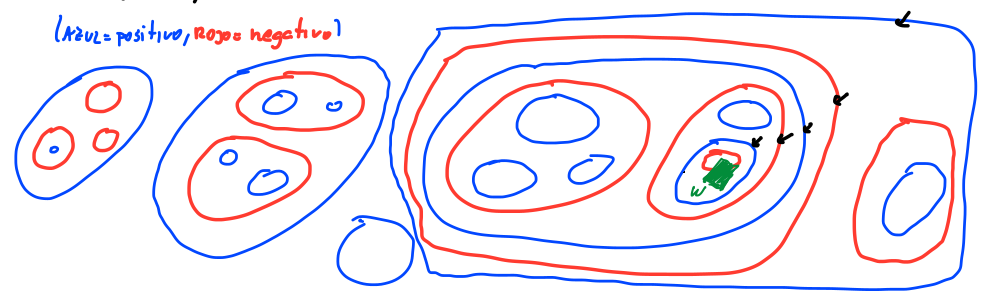
\includegraphics[width=0.75\textwidth]{laminar_set.png}
\end{figure}

Para cualquier $e\in E$, los conjuntos  $A\in \mathcal{F}$ tales que  $e=(s,t)\in \delta^-(A)$ forman una cadena. En efecto si $A, B$ son dos de estos conjuntos, entonces $t\in A\cap B \neq \emptyset$ y como $\mathcal{F}$ es una familia laminar queda que $A\subseteq B$ o $B\subseteq A$ (si no serían conjuntos intersectantes).
Luego para cada $e$, los conjuntos $A$ tales que $e\in \delta^-(A)$ se pueden enumerar tal que $A_1\subseteq A_2 \subseteq \dots A_k$ y los signos de $A_1, A_2, \dots, A_k$ se alternan por  definición. Llamando $\mathcal{F}_+$ y $\mathcal{F}_-$ a los conjuntos de $\mathcal{F}$ positivos y negativos se se tiene: 
\begin{align*}
    \sum_{A\in \mathcal{F}}\text{signo}(A)M_{e,A}=\sum_{A\in \mathcal{F}_{+}}M_{e,A}-\sum_{A\in \mathcal{F}_{+}}M_{e,A}\in\{-1,0,1\}, \; \forall e \in E.
\end{align*}
Luego por Ghoulia-Houri se tiene que la matriz $M$ es TU.

\item Sea $G=(V,E)$ un digrafo. Demuestre que para todo par de conjuntos $A, B\subseteq V$ y todo arco $e=(s,t)\in E$, se tiene la siguiente desigualdad
$$\IV{e\in \delta^-(A\cup B)}+\IV{e\in \delta^-(A\cap B)}-\IV{e\in \delta^-(A)}-\IV{e\in \delta^-(B)} \leq 0$$
donde $\IV{p}=1$ si $p$ es verdadero, y $\IV{p}=0$ en otro caso.
Concluya que para toda función $w\colon E \to \RR_+$, la función $f\colon 2^V\to \RR$ dada por $f(X)=w(\delta^-(X)) = \sum_{e\in \delta^-(X)}w_e$ es submodular.

\textbf{Solución}

Para demostrar la desigualdad anterior basta con ver los casos desfavorables, es decir, en donde el lado positivo se activa ya que de esta manera la expresión podría llegar a ser estrictamente positiva. Si $e=(s,t)\in\delta^{-}(A\cap B)$ para $A, B \subseteq V$ se tiene que $s\notin A\cap B$ y $t\in A\cap B$, esto implica que $t\in A$ y $t\in B$, además,  se cumple solo uno de los siguientes casos, $s\in A\setminus B$, $s\in B\setminus A$ o $s\notin A\cup B$. Si se cumple alguno de los primeros dos casos entonces $e\not\in \delta^{-}(A\cup B)$ y se activa un término negativo por lo que la suma es 0. Si se cumple el tercer caso se tiene $e\in\delta^{-}(A\cup B), e\in\delta^{-}(A), e\in\delta^{-}(B)$ por lo que todos los elementos de la desigualdad se activan y la suma es 0.

Por otro lado, si $e\notin \delta^{-}(A\cap B)$ pero $e\in\delta^{-}(A\cup B)$, se tiene que $s\notin A\cup B$ y se cumple solo uno de los siguientes casos  $t\in A\setminus B$, $t\in B\setminus A$. En ambos casos, se activa un término positivo y un término negativo por lo que la suma es 0.

Por último nos queda demostrar que $f$ es una función submodular, en efecto para cualquier $A, B \subseteq V$,
\begin{align*}
    & f(A\cup B)+f(A\cap B)-f(A)-f(B)
    \\ 
    &=\sum_{e\in \delta^{-}(A\cup B)}w_{e}+\sum_{e\in \delta^{-}(A\cap B)}w_{e}-\sum_{e\in \delta^{-}(A)}w_{e}-\sum_{e\in \delta^{-}(B)}w_{e}\\
    &= \sum_{e\in E}\underbrace{w_{e}}_{\geq 0}\underbrace{\bigg(\IV{e\in \delta^-(A\cup B)}+\IV{e\in \delta^-(A\cap B)}-\IV{e\in \delta^-(A)}-\IV{e\in \delta^-(B)}\bigg)}_{\leq 0} \leq 0,
\end{align*}
se concluye que $f$ es submodular.
\end{enumerate}

\noindent \textbf{Parte II (30 puntos).} \\
\textbf{Nota}: para hacer esta parte recomiendo basarse en las clases 19/20 del curso.\\

Sea $G=(V,E)$ un digrafo y sea $r\in V$ un nodo raiz. Un $r$-conector es cualquier subconjunto $F$ de arcos de $E$ tal que para cada nodo $v\in V$ existe un $r$-$v$ camino dirigido en $F$. Supongamos para evitar conjuntos vacíos que el conjunto $E$ en si mismo es $r$-conector. Defina
$$Q=\{x\in \RR^E\colon x(\delta^-(S))\geq 1, \forall\, \emptyset \neq S\subseteq V\setminus \{r\}, x\geq 0\}$$
El objetivo de este problema es demostrar que $Q=\text{conv}\{\chi^F\colon F\text{ es $r$-conector}\}+\RR_+^E$. Es fácil ver (no lo demuestre) que demostrar la igualdad anterior equivale a demostrar que $Q$ es un poliedro entero. Para hacerlo, demostraremos que el sistema que define a $Q$ es TDI (eso es suficiente pues el vector lado derecho es entero).

Sea $c\in \ZZ^E$ tal que el problema $(P)=\min \{c^Tx\colon x\in Q\}$ tenga solución finita. 
\begin{enumerate}[(a)]
\item (5 puntos) Escriba el dual $(D)$ del problema $(P)$, en variables $(y_S\colon \emptyset \neq S \subseteq V\setminus \{r\}$).

\textbf{Solución}\\
El primal y dual respectivamente:
\begin{align*}
	(P(c)) \min c^{T}x && (D(c)) \max \sum_{\emptyset \neq S\subseteq V\setminus\{r\}}y_{S}\\
	x(\delta^{-}(S))&\geq 1 \;\forall \emptyset \neq S\subseteq V\setminus\{r\} &   \sum_{S: e\in\delta^{-}(S)}y_{S}&\leq c_{e} \; \forall e \in E\\
	x_{e}&\geq 0 \;\forall e \in E &  y_{S}&\geq 0 \;\forall \emptyset \neq S\subseteq V\setminus\{r\}\\
\end{align*}

\item (15 puntos) Llame $y^*$ a una solución óptima de $(D)$ que minimice el potencial $\Psi(y)=\sum_{S} y_S |S||V\setminus S|$. (Existe pues $(P)$ tiene solución finita, y hay un número finito de vértices en el poliedro dual). Demuestre que $y^*$ tiene soporte laminar (es decir, que los conjuntos asociados a coordenadas no nulas de $y^*$ son una familia laminar).\\
\textbf{Indicación:} Al hacer el descruce, considere un par de conjuntos $A$ y $B$ intersectantes y asegúrese que $A\cap B$ y $A\cup B$ indiquen coordenadas del vector $y$.
Use (aunque no la haya hecho) el ejercicio ($f$) de la parte I. 

\textbf{Solución}\\
Consideremos una solución dual óptima $y^{*}$ que minimiza el potencial $\Psi (y)=\sum_{S}y_{S}|S||V\setminus S|$ y sea $\mathcal{L}$ su soporte, es decir, $\mathcal{L}=\{S: y^{*}_{S}>0\}$. Para probar que $\mathcal{L}$ es  laminar utilizaremos la técnica del descruce para construir una solución dual óptima $\hat{y}$ con mejor potencial, lo que nos llevará a una contradicción.

Supondremos que $\mathcal{L}$ no es una familia laminar, esto significa que existen $A, B \in \mathcal{L}$ que son intersectantes, es decir, $A\setminus B, B\setminus A, A\cap B$ son todos no vacíos, luego, consideremos $\hat{y}=
\begin{cases} y^{*}_{S} &  S \notin \{A,B, A\cup B, A\cap B\}\\ y^{*}_{S}-\epsilon & S \in \{A,B\}\\ y^{*}_{S}+\epsilon & S \in \{A\cup B, A\cap B\}
\end{cases}$, con $0<\epsilon\leq \min\{y^{*}_{A}, y^{*}_{B}\}$, de esta manera $\hat{y}$ es no negativo.

\textbf{Paso 1:} Veamos que $\hat{y}$ es dual factible. Si la resta del lado izquierdo de la primera restricción entre  $\hat{y}$ e $y^{*}$ es no positiva entonces $\hat{y}$ es factible, en efecto:
\begin{align*}
\sum_{S:e\in\delta^{-}(S)}\hat{y}_{S}-y^{*}_{S} = \epsilon\bigg(\IV{e\in \delta^{-}(A\cup B)}+\IV{e\in \delta^{-}(A\cap B)}-\IV{e\in \delta^{-}(A)}-\IV{e\in \delta^{-}(B)}\bigg).
\end{align*}
Por P1.f se tiene que la expresión anterior es no positiva, por tanto $\hat{y}$ es dual factible.

\textbf{Paso 2:} Veamos que $\hat{y}$ es dual óptimo, en efecto, como la función objetivo es sumar sobre las componentes de un vector, donde a dos de estos componentes le sumamos $\epsilon$ y a otros dos le restamos $\epsilon$ se tiene que la suma sobre $\hat{y}$ es igual a la suma sobre $y^{*}$.


\textbf{Paso 3:} Veamos que $\hat{y}$ tiene menor potencial que $y^{*}$. En efecto: \begin{align*}
    \Psi(\hat{y})-\Psi(y^{*}) &= \epsilon\bigg(|A\cup B||V\setminus A\cup B|+|A\cap B||V\setminus A\cap B|-|A||V\setminus A|-|B||V\setminus B| \bigg) \\
    &=-2\epsilon|A\setminus B||B\setminus A|
\end{align*}
y esto es menor que $0$ pues $A\setminus B$ y $B\setminus A$ son no vacíos, por ende $\mathcal{L}$ debe ser una familia laminar.

\item (10 puntos) Concluya que el sistema que define a $Q$ es totalmente dual integral.\\
\textbf{Indicación:} Use el resultado del ejercicio ($e$) de la parte I, aunque no lo haya hecho en su tarea.

\textbf{Solución}

El dual restrigido $D^{'}(c)$ al soporte de $y$ se puede escribir de la siguiente forma:

\begin{align*}
	(D^{'}(c))\quad \max \sum_{S\in \mathcal{L}}y_{S}\\
    My&\leq c\\
	y_{S}&\geq 0 \;\forall S\in \mathcal{L},
\end{align*}
donde $M\in\{0,1\}^{E\times \mathcal{L}}$ es tal que $M_{e, S} = 1$ si y solo si $e\in \delta^{-}(S)$. Por P1.e se sabe que $M$ es TU, por lo que si consideramos $c\in \mathbb{Z}^{E}$ se tiene que el área factible de $D^{'}(c)$ es poliedro integral. Así que cuando $P(c)$ tiene óptimo finito, $D(c)$ y $D'(c)$ también y este se alcanza en un vértice $\bar{y}$ de $D^{'}(c)$ que es entero. Como el óptimo de $D(c)$ es factible en $D'(c)$ se concluye que $\bar{y}$ es óptimo en $D(c)$, y luego el sistema original es TDI.

\end{enumerate}

\end{document}
	
	


